\documentclass[a4paper]{article}
\usepackage{geometry}
\usepackage{graphicx}
\usepackage{natbib}
\usepackage{amsmath}
\usepackage{amssymb}
\usepackage{amsthm}
\usepackage{paralist}
\usepackage{epstopdf}
\usepackage{tabularx}
\usepackage{longtable}
\usepackage{multirow}
\usepackage{multicol}
\usepackage[hidelinks]{hyperref}
\usepackage{fancyvrb}
\usepackage{float}
\usepackage{paralist}
\usepackage[svgname]{xcolor}
\usepackage{enumerate}
\usepackage{array}
\usepackage{times}
\usepackage{url}
\usepackage{fancyhdr}
\usepackage{comment}
\usepackage{environ}
\usepackage{times}
\usepackage{textcomp}
\usepackage{caption}
\usepackage{bbm}
\usepackage{enumitem}
\usepackage{algorithm}
\usepackage{algpseudocode}
\usepackage{caption}
\usepackage{subcaption}
\usepackage{tikz}


\urlstyle{rm}

\setlength\parindent{0pt} % Removes all indentation from paragraphs
\theoremstyle{definition}
\newtheorem{definition}{Definition}[]
\newtheorem{conjecture}{Conjecture}[]
\newtheorem{example}{Example}[]
\newtheorem{theorem}{Theorem}[]
\newtheorem{lemma}{Lemma}
\newtheorem{proposition}{Proposition}
\newtheorem{corollary}{Corollary}

\floatname{algorithm}{Procedure}
\renewcommand{\algorithmicrequire}{\textbf{Input:}}
\renewcommand{\algorithmicensure}{\textbf{Output:}}
\newcommand{\abs}[1]{\lvert#1\rvert}
\newcommand{\norm}[1]{\lVert#1\rVert}
\newcommand{\RR}{\mathbb{R}}
\newcommand{\CC}{\mathbb{C}}
\newcommand{\Nat}{\mathbb{N}}
\newcommand{\br}[1]{\{#1\}}
\DeclareMathOperator*{\argmin}{arg\,min}
\DeclareMathOperator*{\argmax}{arg\,max}
\renewcommand{\qedsymbol}{$\blacksquare$}

\definecolor{dkgreen}{rgb}{0,0.6,0}
\definecolor{gray}{rgb}{0.5,0.5,0.5}
\definecolor{mauve}{rgb}{0.58,0,0.82}

\newcommand{\Var}{\mathrm{Var}}
\newcommand{\Cov}{\mathrm{Cov}}

\newcommand{\vc}[1]{\boldsymbol{#1}}
\newcommand{\xv}{\vc{x}}
\newcommand{\Sigmav}{\vc{\Sigma}}
\newcommand{\alphav}{\vc{\alpha}}
\newcommand{\muv}{\vc{\mu}}

\newcommand{\red}[1]{\textcolor{red}{#1}}

\def\x{\mathbf x}
\def\y{\mathbf y}
\def\w{\mathbf w}
\def\v{\mathbf v}
\def\E{\mathbb E}
\def\V{\mathbb V}
\def\ind{\mathbbm 1}

% TO SHOW SOLUTIONS, include following (else comment out):
\newenvironment{soln}{
	\leavevmode\color{blue}\ignorespaces
}{}

\hypersetup{
	%    colorlinks,
	linkcolor={red!50!black},
	citecolor={blue!50!black},
	urlcolor={blue!80!black}
}

\geometry{
	top=1in,            % <-- you want to adjust this
	inner=1in,
	outer=1in,
	bottom=1in,
	headheight=3em,       % <-- and this
	headsep=2em,          % <-- and this
	footskip=3em,
}


\pagestyle{fancyplain}
\lhead{\fancyplain{}{Homework 6}}
\rhead{\fancyplain{}{CS 760 Machine Learning}}
\cfoot{\thepage}

\title{\textsc{Homework 6}} % Title


\author{
	Nick Boddy \\
	nboddy \\
	GitHub repo: github.com/Nick-Boddy/CS760-HW6-GAN-BayesNet \\
} 

\date{2023-11-17}

\begin{document}
	
	\maketitle 
	
        \textbf{Instructions:}
        Use this latex file as a template to develop your homework. Submit your homework on time as a single pdf file. Please wrap your code and upload to a public GitHub repo, then attach the link below the instructions so that we can access it. Answers to the questions that are not within the pdf are not accepted. This includes external links or answers attached to the code implementation. Late submissions may not be accepted. You can choose any programming language (i.e. python, R, or MATLAB). Please check Piazza for updates about the homework. It is ok to share the results of the experiments and compare them with each other.
        \vspace{0.1in}
	
	\section{Implementation: GAN (50 pts)}
	In this part, you are expected to implement GAN with MNIST dataset. We have provided a base jupyter notebook (gan-base.ipynb) for you to start with, which provides a model setup and training configurations to train GAN with MNIST dataset.
	
	\begin{enumerate} [label=(\alph*)]
		\item Implement training loop and report learning curves and generated images in epoch 1, 50, 100. Note that drawing learning curves and visualization of images are already implemented in provided jupyter notebook. \hfill (20 pts)
		
		\begin{algorithm}
			\caption{Training GAN, modified from \cite{goodfellow2014generative}}\label{alg:GAN}
			\begin{algorithmic}
				\Require $m$: real data batch size, $n_{z}$: fake data batch size
				\Ensure Discriminator $D$, Generator $G$
				
				\For{number of training iterations}
				
				\State{$\#$ Training discriminator}
				\State{Sample minibatch of $n_{z}$ noise samples $\{z^{(1)}, z^{(2)}, \cdots, z^{(n_{z})}\}$ from noise prior $p_{g}(z)$}
				\State{Sample minibatch of $\{x^{(1)}, x^{(2)}, \cdots, x^{(m)}\}$}
				\State{Update the discriminator by ascending its stochastic  gradient:
					$$\nabla_{\theta_{d}} \big ( \cfrac{1}{m}  \sum_{i=1}^{m}  \log D(x^{(i)})  + \cfrac{1}{n_{z}} \sum_{i=1}^{n_{z}}  \log (1-D(G(z^{(i)})))\big )$$
				}
				
				\State{$\#$ Training generator}
				\State{Sample minibatch of $n_{z}$ noise samples $\{z^{(1)}, z^{(2)}, \cdots, z^{(n_{z})}\}$ from noise prior $p_{g}(z)$}
				\State{Update the generator  by ascending its stochastic  gradient:
					$$\nabla_{\theta_{g}}  \cfrac{1}{n_{z}} \sum_{i=1}^{n_{z}}  \log D(G(z^{(i)}))\big )$$
				}
				\EndFor
				
				\State{$\#$ The gradient-based updates can use any standard gradient-based learning rule. In the base code, we are using Adam optimizer \citep{kingma2014adam}}
			\end{algorithmic}
		\end{algorithm}
		
		Expected results are as follows.
		
		\begin{figure}[H]
			\centering
			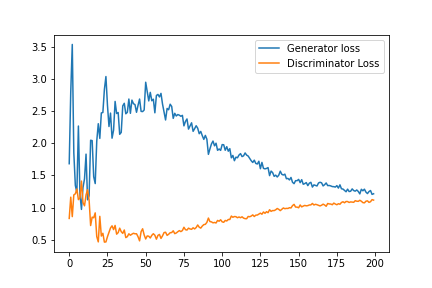
\includegraphics[width=0.7\textwidth]{gan_q1_loss.png}
			\caption{Learning curve}
			\label{fig:gan_q1_loss}
		\end{figure}
		
		\begin{figure}[H]
			\centering
			\begin{subfigure}[b]{0.3\textwidth}
				\centering
				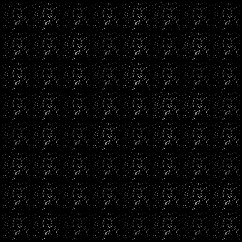
\includegraphics[width=\textwidth]{gan_q1_epoch1.png}
				\caption{epoch 1}
			\end{subfigure}
			\hfill
			\begin{subfigure}[b]{0.3\textwidth}
				\centering
				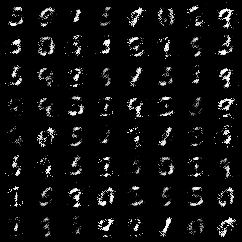
\includegraphics[width=\textwidth]{gan_q1_epoch50.png}
				\caption{epoch 50}
			\end{subfigure}
			\hfill
			\begin{subfigure}[b]{0.3\textwidth}
				\centering
				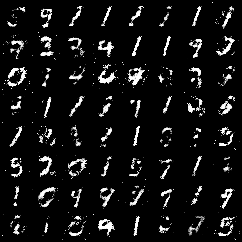
\includegraphics[width=\textwidth]{gan_q1_epoch100.png}
				\caption{epoch 100}
			\end{subfigure}
			\caption{Generated images by $G$}
			\label{fig:three graphs}
		\end{figure}
		
		
		\begin{soln}
			
			\begin{figure}[H]
				\centering
				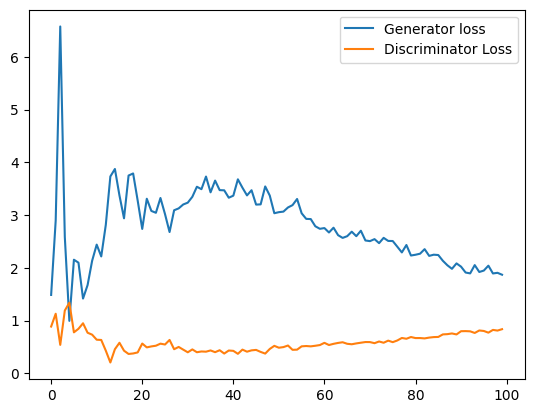
\includegraphics[width=4in]{1a_curve.png}
				\caption{My learning curve}
				\label{fig:gan_q1_loss}
			\end{figure}
			
			\begin{figure}[H]
				\centering
				\begin{subfigure}[b]{0.3\textwidth}
					\centering
					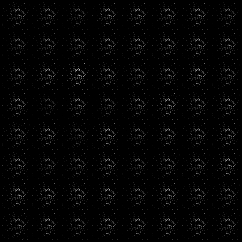
\includegraphics[width=\textwidth]{1a_e1.png}
					\caption{epoch 1}
				\end{subfigure}
				\hfill
				\begin{subfigure}[b]{0.3\textwidth}
					\centering
					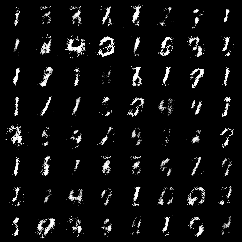
\includegraphics[width=\textwidth]{1a_e50.png}
					\caption{epoch 50}
				\end{subfigure}
				\hfill
				\begin{subfigure}[b]{0.3\textwidth}
					\centering
					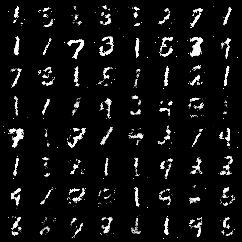
\includegraphics[width=\textwidth]{1a_e100.png}
					\caption{epoch 100}
				\end{subfigure}
				\caption{My generated images from $G$}
				\label{fig:three graphs}
			\end{figure}
		\end{soln}
		
		
		
		\item Replace the generator update rule as the original one in the slide,\\
		``Update the generator by descending its stochastic gradient:
		
		$$\nabla_{\theta_{g}}  \cfrac{1}{n_{z}}  \sum_{i=1}^{n_{z}}\log (1-D(G(z^{(i)})))\big )$$
		"
		, and report learning curves and generated images in epoch 1, 50, 100. Compare the result with (a). Note that it may not work. If training does not work, explain why it doesn't work. \\
        You may find this helpful: https://jonathan-hui.medium.com/gan-what-is-wrong-with-the-gan-cost-function-6f594162ce01
		\hfill (10 pts)
		
		\begin{soln}
			\begin{figure}[H]
				\centering
				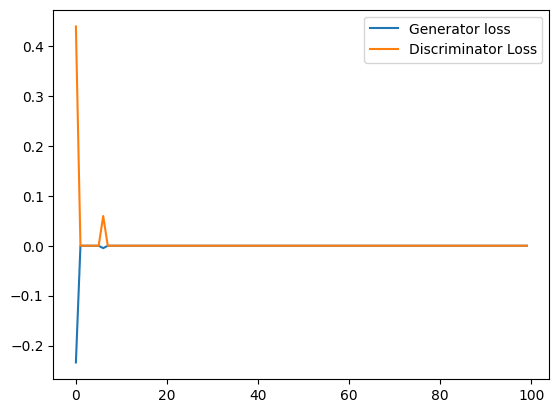
\includegraphics[width=4in]{1b_curve.png}
				\caption{My learning curve}
				\label{fig:gan_q1_loss}
			\end{figure}
			
			\begin{figure}[H]
				\centering
				\begin{subfigure}[b]{0.3\textwidth}
					\centering
					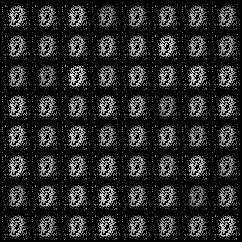
\includegraphics[width=\textwidth]{1b_e1.png}
					\caption{epoch 1}
				\end{subfigure}
				\hfill
				\begin{subfigure}[b]{0.3\textwidth}
					\centering
					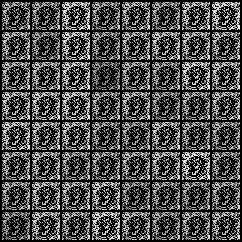
\includegraphics[width=\textwidth]{1b_e50.png}
					\caption{epoch 50}
				\end{subfigure}
				\hfill
				\begin{subfigure}[b]{0.3\textwidth}
					\centering
					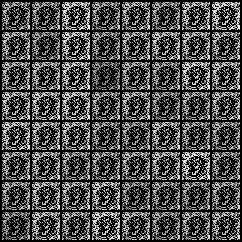
\includegraphics[width=\textwidth]{1b_e100.png}
					\caption{epoch 100}
				\end{subfigure}
				\caption{My generated images from $G$ using an altered update rule}
				\label{fig:three graphs}
			\end{figure}
			
			The results of using this altered rule for updating the generator clearly does not result in realistic images. This makes sense, since the new update rule of descending $\nabla_{\theta_{g}}  \cfrac{1}{n_{z}}  \sum_{i=1}^{n_{z}}\log (1-D(G(z^{(i)})))\big )$ diminishes when the discriminator improves. Even though conceptually the $\theta_{g}$ that minimizes $\cfrac{1}{n_{z}}  \sum_{i=1}^{n_{z}}\log (1-D(G(z^{(i)})))\big )$ is the same $\theta_{g}$ that maximizes $\cfrac{1}{n_{z}} \sum_{i=1}^{n_{z}}  \log D(G(z^{(i)}))\big )$, when considering the backpropagating gradients, the former values diminish to the point where the gradient vanishes, whereas the latter (which is used in part a), does not vanish (but could possibly be unstable).
			
		\end{soln}
		
		\item Except the method that we used in (a), how can we improve training for GAN? Implement that and report your setup, learning curves, and generated images in epoch 1, 50, 100.
        This question is an open-ended question and you can choose whichever method you want.
		\hfill (20 pts)
		
		\begin{soln}
			I've tried a couple modifications, some more successful than others. I tried altering the labels to be more smooth in training, with a $0.9$ for real images instead of $1$, and $0.1$ for fake images instead of $0$.
		\end{soln}
		
	\end{enumerate}

\section{Directed Graphical Model [25 points]}
Consider the directed graphical model (aka Bayesian network) in Figure~\ref{fig:bn}.
\begin{figure}[H]
    \centering
    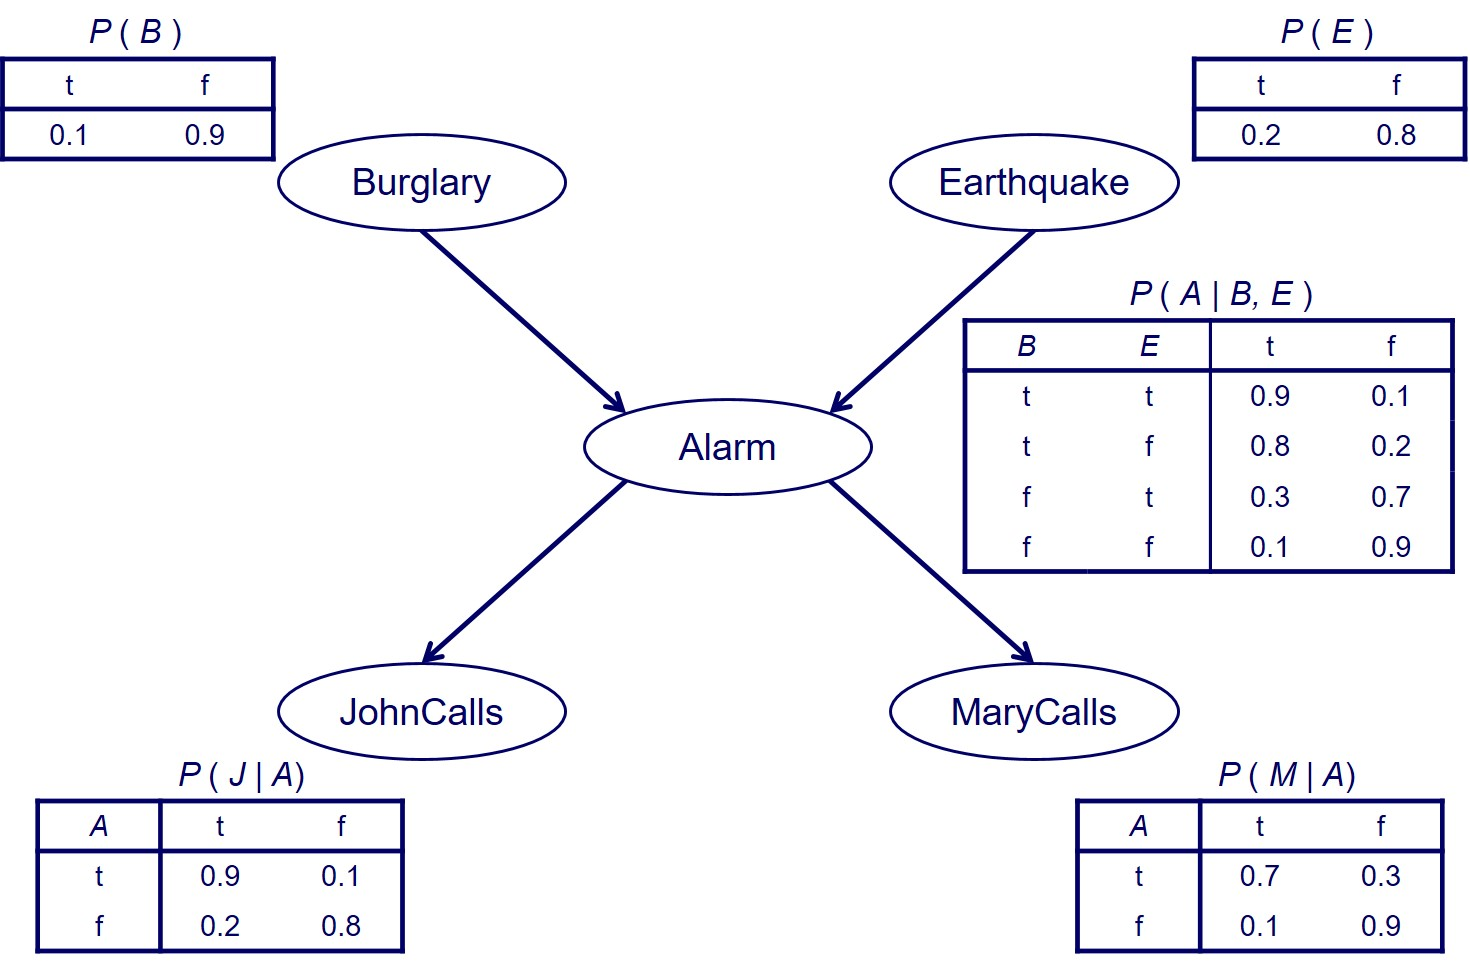
\includegraphics[width=0.8\textwidth]{BN.jpeg}
    \caption{A Bayesian Network example.}
    \label{fig:bn}
\end{figure}
Compute $P(B=t \mid E=f,J=t,M=t)$ and $P(B=t \mid E=t,J=t,M=t)$. (10 points for each) These are the conditional probabilities of a burglar in your house (yikes!) when both of your neighbors John and Mary call you and say they hear an alarm in your house, but without or with an earthquake also going on in that area (what a busy day), respectively.

\begin{soln}
	$$P(B=t \mid E=f,J=t,M=t)$$
	$$ = P(B \mid \neg E, J, M) = \frac{P(B, \neg E, J, M)}{P(\neg E, J, M)}$$
	$$ = \frac{P(B, \neg E, J, M)}{P(B, \neg E, J, M) + P(\neg B, \neg E, J, M)}$$
	$$P(B, \neg E, J, M) = \sum_{a \in \{A, \neg A\}} P(B) P(\neg E) P(a | B, \neg E) P(J | a) P(M | a)$$
	$$ = (0.1)(0.8)(0.8)(0.9)(0.7) + (0.1)(0.8)(0.2)(0.2)(0.1) = 0.04064$$
	$$P(\neg B, \neg E, J, M) = \sum_{a \in \{A, \neg A\}} P(\neg B) P(\neg E) P(a | \neg B \neg E) P(J | a) P(M | a)$$
	$$ = (0.9)(0.8)(0.1)(0.9)(0.7) + (0.9)(0.8)(0.9)(0.2)(0.1) = 0.05832$$
	$$P(B \mid \neg E, J, M) = \frac{0.04064}{0.04064 + 0.05832} = 0.410670978$$
	\\ \\
	$$P(B=t \mid E=t,J=t,M=t)$$
	$$ = P(B \mid E, J, M) = \frac{P(B, E, J, M)}{P(E, J, M)}$$
	$$ = \frac{P(B, E, J, M)}{P(B, E, J, M) + P(\neg B, E, J, M)}$$
	$$P(B, E, J, M) = \sum_{a \in \{A, \neg A\}} P(B) P(E) P(a | B, E) P(J | a) P(M | a)$$
	$$ = (0.1)(0.2)(0.9)(0.9)(0.7) + (0.1)(0.2)(0.1)(0.2)(0.1) = 0.01138$$
	$$P(\neg B, E, J, M) = \sum_{a \in \{A, \neg A\}} P(\neg B) P(E) P(a | \neg B, E) P(J | a) P(M | a)$$
	$$ = (0.9)(0.2)(0.3)(0.9)(0.7) + (0.9)(0.2)(0.7)(0.2)(0.1) = 0.03654$$
	$$P(B \mid E, J, M) = \frac{0.01138}{0.01138 + 0.03654} = 0.237479132$$
	\\ \\
	$$P(B \mid \neg E, J, M) \approx 0.411$$
	$$P(B \mid E, J, M) \approx 0.237$$
\end{soln}


\section{Chow-Liu Algorithm [25 pts]}
Suppose we wish to construct a directed graphical model for 3 features $X$, $Y$, and $Z$ using the Chow-Liu algorithm. We are given data from 100 independent experiments where each feature is binary and takes value $T$ or $F$. Below is a table summarizing the observations of the experiment:

\begin{table}[H]
        \centering
                \begin{tabular}{cccc}
                           $X$ & $Y$ & $Z$ & Count \\
                                \hline
                                T & T & T & 36 \\
                                \hline
                                T & T & F & 4 \\
                                \hline
                                T & F & T & 2 \\
                                \hline
                                T & F & F & 8 \\
                                \hline
                                F & T & T & 9 \\
                                \hline
                                F & T & F & 1 \\
                                \hline
                                F & F & T & 8 \\
                                \hline
                                F & F & F & 32 \\
                                \hline
                \end{tabular}
\end{table}

\begin{enumerate}
	\item Compute the mutual information $I(X, Y)$ based on the frequencies observed in the data. (5 pts)
	
	\begin{soln}
		$$I(X, Y) = \sum_{x \in \{X, \neg X\}} \sum_{y \in \{Y, \neg Y\}} P(x,y) \log_2 \frac{P(x,y)}{P(x) P(y)}$$
		$$ = 0.4 \log_2 \frac{0.4}{0.5 \times 0.5} + 0.1 \log_2 \frac{0.1}{0.5 \times 0.5} + 0.1 \log_2 \frac{0.1}{0.5 \times 0.5} + 0.4 \log_2 \frac{0.4}{0.5 \times 0.5}$$
		$$ \approx 0.2781$$
	\end{soln}
	
	\item Compute the mutual information $I(X, Z)$ based on the frequencies observed in the data. (5 pts)
	
	\begin{soln}
		$$I(X, Z) = \sum_{x \in \{X, \neg X\}} \sum_{z \in \{Z, \neg Z\}} P(x,z) \log_2 \frac{P(x,z)}{P(x) P(z)}$$
		$$ = 0.38 \log_2 \frac{0.38}{0.5 \times 0.55} + 0.12 \log_2 \frac{0.12}{0.5 \times 0.45} + 0.17 \log_2 \frac{0.17}{0.5 \times 0.55} + 0.33 \log_2 \frac{0.33}{0.5 \times 0.45}$$
		$$ \approx 0.1328$$
	\end{soln}
	
	\item Compute the mutual information $I(Z, Y)$ based on the frequencies observed in the data. (5 pts)
	
	\begin{soln}
		$$I(Z, Y) = \sum_{z \in \{Z, \neg Z\}} \sum_{y \in \{Y, \neg Y\}} P(z,y) \log_2 \frac{P(z,y)}{P(z) P(y)}$$
		$$ = 0.45 \log_2 \frac{0.45}{0.55 \times 0.5} + 0.1 \log_2 \frac{0.1}{0.55 \times 0.5} + 0.05 \log_2 \frac{0.05}{0.45 \times 0.5} + 0.4 \log_2 \frac{0.4}{0.45 \times 0.5}$$
		$$ \approx 0.3973$$
	\end{soln}
	
	\item Which undirected edges will be selected by the Chow-Liu algorithm as the maximum spanning tree? (5 pts)
	
	\begin{soln}
		The candidate edges are $(X, Y)$, $(X, Z)$ and $(Y, Z)$. The Chow-Liu algorithm first selects the edge with the largest weight (in this case, our edge weights are the mutual information), which will be $(Y, Z)$ with a mutual information of $0.3973$. \\
		The next largest edge will be $(X, Y)$ with a weight of $0.2781$. \\
		The next largest edge is $(X, Z)$ with a weight of $0.1328$, but since adding $(X, Z)$ creates a cycle in the graph, we do not add it. \\ \\
		So the maximum spanning tree generated is $G = \bigg(V := \{X, Y, Z\}, E := \{(Y, Z), (X, Y)\}\bigg)$
	\end{soln}

	\item Root your tree at node $X$, assign directions to the selected edges. (5 pts)
	
	\begin{soln}
		\begin{center}
			\begin{tikzpicture}
				\node[circle, draw] (X) at (1,2) {X};
				\node[circle, draw] (Y) at (0,0) {Y};
				\node[circle, draw] (Z) at (2,0) {Z};
				\draw[->] (X) -- (Y);
				\draw[->] (Y) -- (Z);
			\end{tikzpicture}
		\end{center}
		\[
		P(X) =
		\begin{tabular}{|c  c|}
			\hline
			T & F \\
			\hline
			0.5 & 0.5 \\
			\hline
		\end{tabular}
		\]
		
		\[
		P(Y \mid X) =
		\begin{tabular}{| c | c  c |}
			\hline
			X & T & F \\
			\hline
			T & 0.8 & 0.2 \\
			F & 0.2 & 0.8 \\
			\hline
		\end{tabular}
		\]
		
		\[
		P(Z \mid Y) =
		\begin{tabular}{| c | c  c |}
			\hline
			Y & T & F \\
			\hline
			T & 0.9 & 0.1 \\
			F & 0.2 & 0.8 \\
			\hline
		\end{tabular}
		\]
	\end{soln}
	
\end{enumerate}

	\bibliography{hw6}
	\bibliographystyle{apalike}
\end{document}
